
\subsection{Participants} 
Protocol implementation involves realization of the protocol building blocks as well as providing means of data communication between them. Building blocks are placed at the following locations, which correspond to protocol participants:

\begin{itemize}%[label=$\bullet$]
	\item User software.
	\item License provider software.
	\item Service provider software.
	\item Citadel contract.
\end{itemize}

\begin{flushleft}
Data communication between protocol participants is realized via the following communication modes:
\end{flushleft}

\begin{itemize}%[label=$\bullet$]
	\item Transactions changing the contract state.
	\item Queries against the contract state.
	\item Storing data directly in blockchain by issuing recipient-less transactions.
	\item Retrieving data from blockchain by scanning transactions.
\end{itemize}

\begin{flushleft}
The following diagram illustrates an interaction between protocol participants and indicates the communication means used.
\end{flushleft}

\begin{figure}[h]
	\centering
		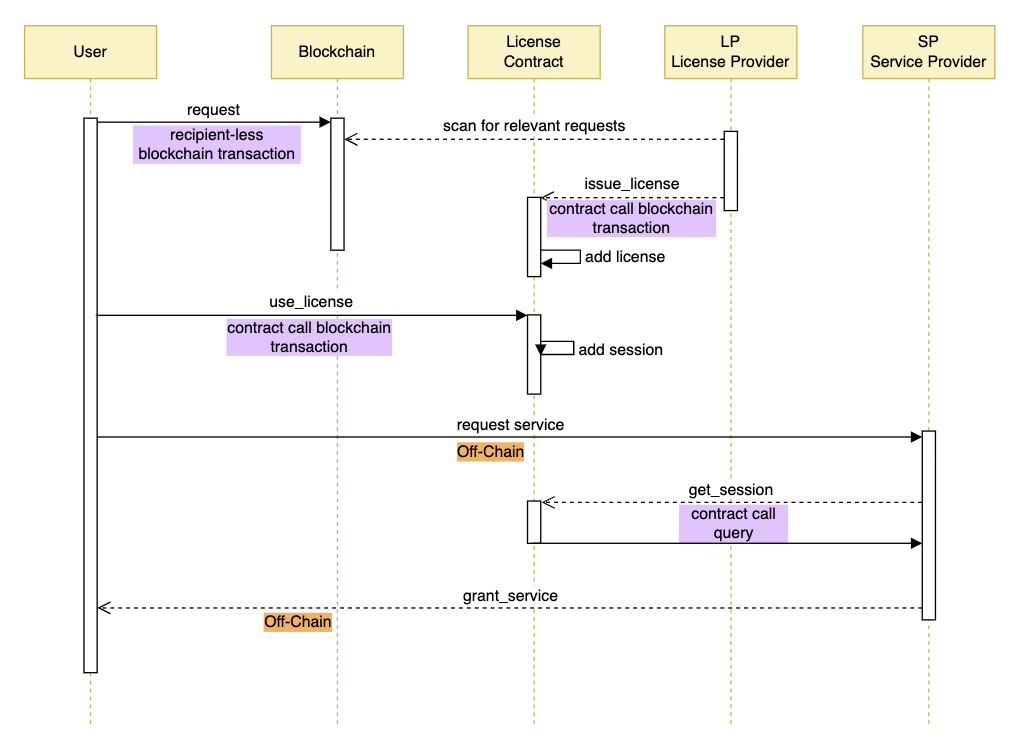
\includegraphics[width=390pt,draft=false]{images/implementation.png}
	\caption{Interaction between protocol participants}
	\label{fig:implementation}
\end{figure}

On the diagram we can see various communication modes being used. Initially, the user publishes recipient-less transaction containing a request as payload into the blockchain. Subsequently, license provider can scan the blockchain for transactions containing relevant requests. License provider can obtain requests via other routes as well, for example via http or email, passing requests on blockchain is only one of possible ways. Once License Provider gets a hold of a request, it can perform appropriate verification and issue a license. Issuing a license involves another mode of communication - a smart contract transaction call. Smart contract transaction call is also a blockchain transaction, yet to not to confuse the reader, we show it on the diagram while skipping the detail that blockchain is involved.

The diagram illustrates following flow of data and interactions between participants:

\begin{itemize}%[label=$\bullet$]
	\item User sends request to the License Provider by issuing a blockchain transaction.
	\item License provider scans blockchain for requests and obtains the request.
	\item License provider, upon necessary verification, issues a license.
	\item License provider sends the license to License Contract via a smart contract call transaction.
	\item User obtains licenses for a given block-height range.
	\item User filters out licenses addressed to her or him.
	\item User calculates a proof.
	\item User calls use-license to redeem a license, via a smart contract call.
	\item License Contract attempts to verify the proof and, if verified, adds a new session to a list of sessions.
	\item User requests a service from a Service Provider (off-chain).
	\item Service Provider asks contract for a session.
	\item Service Provider grants service to the user (off-chain).
\end{itemize}


\subsection{License Contract}

\begin{flushleft}
License contract maintains state consisting of the following data:
\end{flushleft}

\begin{itemize}%[label=$\bullet$]
	\item List of sessions.
	\item Map of licenses and their positions in the Merkle tree.
	\item Merkle tree of license hashes.
\end{itemize}


\begin{flushleft}
Contract provides the following methods:
\end{flushleft}

\begin{itemize}%[label=$\bullet$]
	\item \textit{issue-license}
	\item \textit{get-licenses}
	\item \textit{use-license}
	\item \textit{get-session}
\end{itemize}


\begin{flushleft}
\textit{issue-license} adds a license to a Merkle tree of licenses. \textit{get-licenses} provides a list of new licenses added in a given block-height range \textit{use-license} attempts to verify the proof and, if verified, adds a new session to a list of sessions, nullifies the license in the Merkle tree. \textit{get-session} finds a session in a list of sessions and returns it to the caller.
\end{flushleft}


